\section{Introduction}

In this chapter we apply the methodology illustrated in the previous chapter to the concrete EUR market case in order to produce a new proposal for the EUR Rate Curve Framework. Obviously we do not claim that our choices are the best solution to any problems, being related to many factors as the particular market situation we have experienced during last years. 

We will calibrate five curves: $C_{ON}, C_{1M}, C_{3M}, C_{6M}, C_{12M}$ whose underlying indexes are Eonia, Euribor 1M, Euribor 3M, Euribor 6M, Euribor 12M respectively. Actually for each curve we will have two calibrations: first an Excel calibration, performed with market quotes and only the synthetic deposits quotes needed to fix the curve over the interval $[t,spot(today)+x]$; secondly a front office system calibration, performed with a set of contribution instruments which includes part or all of the instruments used for the first calibration plus other synthetic interpolated instruments (as explained in section \ref{sec:synthinterp}). Also, the second calibration could be performed with different settings (reference date, interpolation, ...). Let us explain why this double calibration is still used in the actual Banca IMI framework.

Today some hedging practices are still related to the old one-curve world. In particular, instead of using multiple set of hedging instruments (one of each curve) as explained in section \ref{sec:deltas}, a unique set of hedging instruments of different tenors is selected. In order to do thi,s all curves must have the same structure (typically the standard Deposits-Futures-Swaps structure) so that it is straightforward to aggregate bucket by bucket the deltas of different curves. In practice we have a common time grid $T_{1},...,T_{m}$, a common set of calibrating instruments but use different quotes $\{Q_{ij}\}_{j=1,...,m}$ for each curve. Once we compute bucketed deltas, we then aggregate on each pillar as follows:
$$\bar{\Delta}_{j}(t;Q)=\sum_{i=1}^{n}\Delta^{\Pi}_{ij}(t;Q)$$
In this way, it's no more possible to identify the contribution related to each single curve and the hedge can be performed as in the old one-curve framework. This method has at least two big drawbacks: first, it ignores that different tenors have different related instruments; secondly, we have to find a reasonable method to build all curves with the same structure without being in conflict with the homogeneous instruments selection criteria. Here the double calibration plays a fundamental role because we can calibrate curves in Excel using best practices and then contribute to the front office system for each of them a common set of instruments in order to have the same structure for every curve. For example, we can calibrate each $xM$ Euribor curve using only xM tenor instruments and then contribute to the system Deposits of different tenors, 3M futures and 6M swaps for every curve. 

It's not possible with the actual infrastructure to completely avoid the double calibration process (for example, the front office system can't calculate synthetic deposits). Our proposal, instead, is to align as much as possible the two calibrations, in order to have both on Excel and inside the system a set of curves representative of the real market. These obviously imply a change in hedging practices that is still ongoing. Unfortunately some differences between first and second calibration still remains. We illustrate here the main ones.

\subsubsection{Curves reference date}

As discussed in section \ref{sec:synth}, we have to set discounting curve reference date to today (in order to be able to calculate today's value of cash flows). For forwarding curves, instead, we prefer to set reference date to the spot date of calibrating instruments. This is possible on Excel but not inside the front office system where the whole set of curves has reference date equal to today. This is a small inconsistency that still remains.    

\subsubsection{Interpolation scheme and instruments selection}

As discussed in section \ref{sec:deltas} the best compromise between having good forward rates and stable/reasonable deltas calculation seems a bootstrap performed with a Kruger scheme applied on zero rates even if the corresponding forwards rates are not the best ones. In order to weaken their humped behavior, we follow these steps: 
\begin{itemize}
\item we use Hyman scheme on Zero Rates for Excel Calibration in order to have a good curve from a forward rates point of view; this choice produces non-local deltas but we can tolerate it because the main purpose of this calibration is contribution (not sensitivities calculation); the only synthetic instruments used here are deposits.
\item we create the set of contribution instruments including all the calibrating instruments plus a set of synthetic interpolated instruments to obtain a ticker time grid (mostly for the long term part of the curve);
\item finally we use Kruger scheme on zero rates for the second calibration; both synthetic deposits and synthetic interpolated instruments are used here.
\end{itemize}
The result of this process for Euribor 6M Curve (Evaluation Date: 30 October 2015) is shown in Figures \ref{fig:10} and \ref{fig:9}.

\begin{figure}
\centering
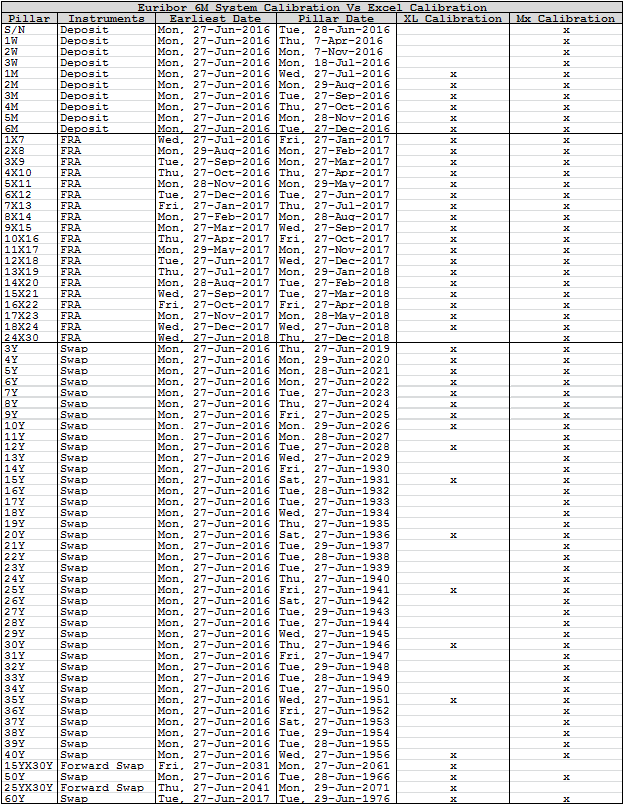
\includegraphics[width=0.7\textwidth]{images/10.png}
\caption{Excel Calibration vs System Calibration for Euribor 6M Curve (Evaluation Date 30 October 2015)}
\label{fig:10}
\end{figure}
\begin{figure}
\centering
\begin{subfigure}[b]{0.7\textwidth}
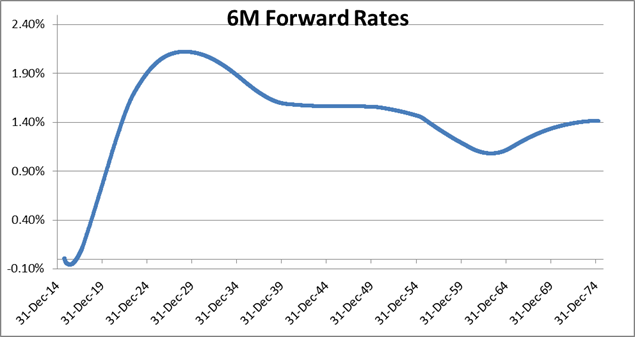
\includegraphics[width=\textwidth]{images/9a.png}
\caption{Hyman on Zero Rates - Synthetic Deposits and Market Instruments (Excel Calibration)}
\label{fig:9a}
\end{subfigure}
\begin{subfigure}[b]{0.7\textwidth}
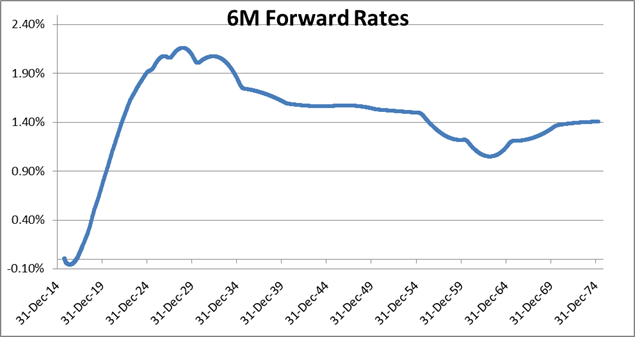
\includegraphics[width=\textwidth]{images/9b.png}
\caption{Kruger on Zero Rates - Synthetic Deposits and Market Instruments}
\label{fig:9b}
\end{subfigure}
\begin{subfigure}[b]{0.7\textwidth}
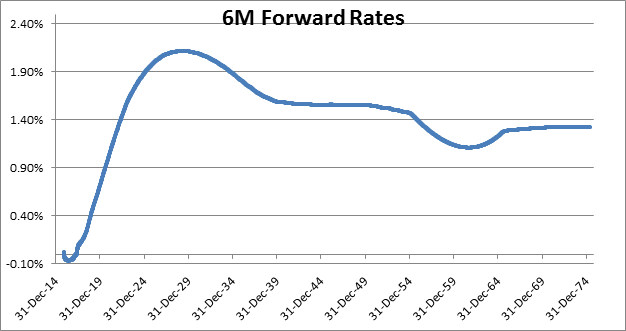
\includegraphics[width=\textwidth]{images/9c.png}
\caption{Kruger on Zero Rates - Synthetic Deposits, Synthetic Interpolated Instruments and Market Instruments (System Calibration)}
\label{fig:9c}
\end{subfigure}
\caption{Excel Calibration vs System Calibration for Euribor 6M Curve (Evaluation Date 30 October 2015)}
\label{fig:9}
\end{figure}

\subsubsection{Synthetic Instruments}
As said before, the Excel calibration is performed using only the necessary synthetic deposits (needed to fix the curve over the interval $[t,spot(today)+x]$) and no other synthetic instruments. Instead the system calibration makes use of synthetic interpolated instruments of two kinds: instruments corresponding to non quoted maturities (as just illustrated) or instruments not quoted at all (example: the market quotes basis swaps but system calibration is performed with swaps, which are preferred for hedging).  

\section{ON Curve}

\subsection{Excel Calibration}

Eonia curve is bootstrapped using the following instruments:
\begin{itemize}
\item ON and TN Deposits in order to set the curve reference date to today's date (these instruments are not properly based on Eonia - the underlying index is the one-day tenor Euribor - thus we are introducing a very small inconsistency);
\item all the available forward starting OIS on ECB dates;
\item spot starting OIS up to 60Y.
\end{itemize}
The ECB OIS are more liquid than spot starting OIS and this is way we always use them when available. There are no synthetic instruments.

The curve structure with corresponding Market RICs is shown in Figure \ref{fig:ONExcel}.

\begin{figure}
\centering
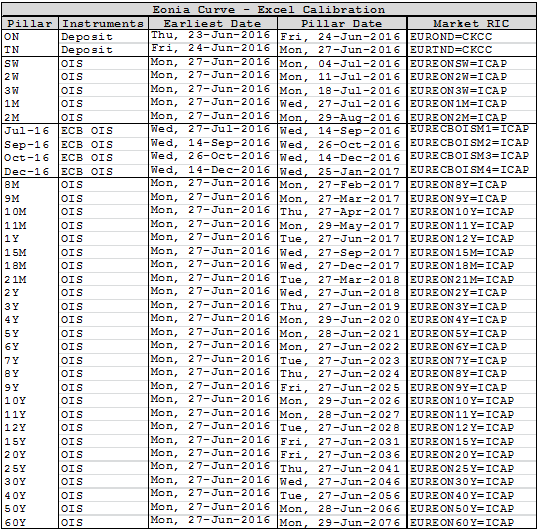
\includegraphics[width=0.58\textwidth]{images/ONExcel.png}
\caption{Bootstrapping instruments selected for Excel calibration of Eonia Curve and corresponding Market RICs (Evaluation Date 30 October 2015)}
\label{fig:ONExcel}
\end{figure}

\subsection{System Calibration}

The curve structure with corresponding Internal RICs is shown in Figure \ref{fig:ONMx}. The contribution instruments (i.e. instruments priced using the Excel curve and then used to perform the system calibration) are listed below:
\begin{itemize}
\item ON, TN, SN Deposits;
\item spot starting OIS up to 60Y.
\end{itemize}
Notice the presence of synthetic interpolated instruments.

\begin{figure}
\centering
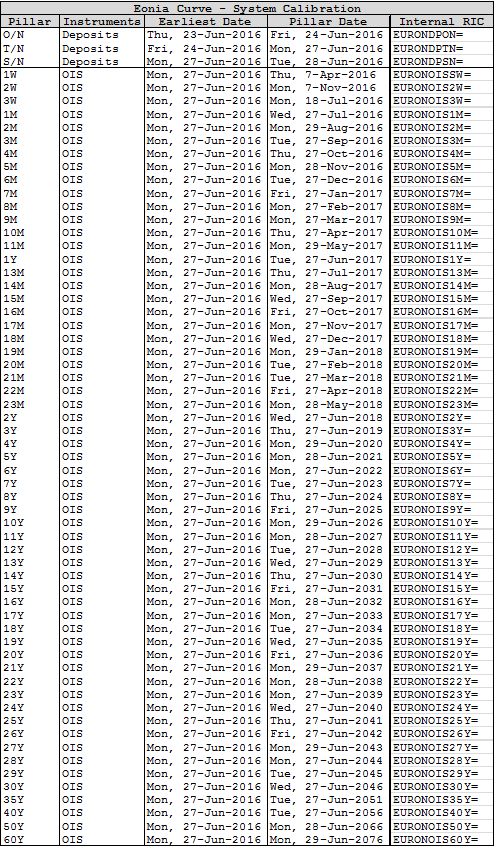
\includegraphics[width=0.58\textwidth]{images/ONMx.png}
\caption{Bootstrapping instruments selected for System calibration of Eonia Curve and corresponding Internal RICs (Evaluation Date 30 October 2015)}
\label{fig:ONMx}
\end{figure}

\section{1M Curve}

\subsection{Excel Calibration}

1M Euribor curve is bootstrapped using the following instruments:
\begin{itemize}
\item SW, 2W, 3W, 1M Synthetic Deposits; 
\item 1M Swap with $Act/360$ convention up to 12M;
\item 1M Swap with $30/360$ convention up to 60Y.
\end{itemize}
The curve structure with corresponding Market RICs is shown in Figure \ref{fig:1MExcel}.

\begin{figure}
\centering
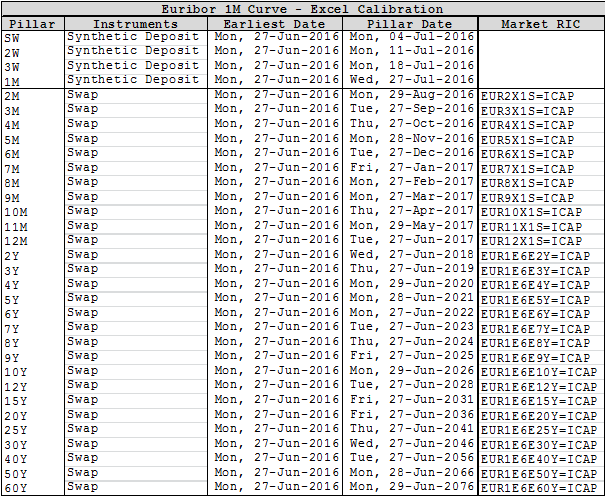
\includegraphics[width=0.58\textwidth]{images/1MExcel.png}
\caption{Bootstrapping instruments selected for Excel calibration of Euribor 1M Curve and corresponding Market RICs (Evaluation Date 30 October 2015)}
\label{fig:1MExcel}
\end{figure}

\subsection{System Calibration}

The curve structure with corresponding Internal RICs is shown in Figure \ref{fig:1MMx}. The contribution instruments are listed below:
\begin{itemize}
\item SN, SW, 2W, 3W, 1M Deposits; 
\item 1M Swap with $Act/360$ convention up to 12M;
\item 1M Swap with $30/360$ convention up to 60Y.
\end{itemize}
Once again we notice the presence of many synthetic interpolated instruments added to have one pillar every three months from 1Y to 3Y maturities and one pillar every year from 3Y to 40Y maturities. 

\begin{figure}
\centering
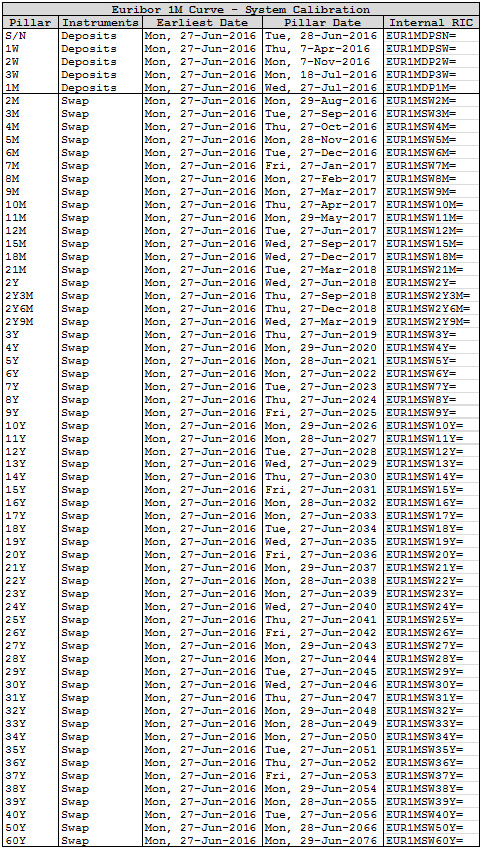
\includegraphics[width=0.58\textwidth]{images/1MMx.png}
\caption{Bootstrapping instruments selected for System calibration of Euribor 1M Curve and corresponding Internal RICs (Evaluation Date 30 October 2015)}
\label{fig:1MMx}
\end{figure}

\section{3M Curve}

\subsection{Excel Calibration}

3M Euribor curve is bootstrapped using the following instruments:
\begin{itemize}
\item 1M, 2M, 3M Synthetic Deposits; 
\item 8 IMM Futures;
\item 3M Swaps up to 60Y.
\end{itemize}
The curve structure with corresponding Market RICs is shown in Figure \ref{fig:3MExcel}.

\begin{figure}
\centering
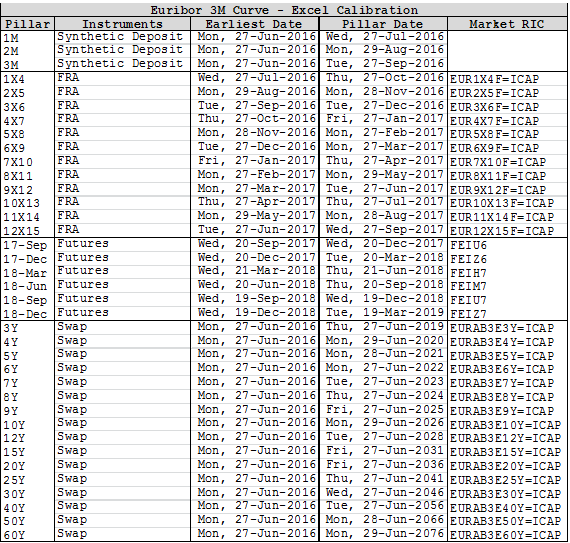
\includegraphics[width=0.58\textwidth]{images/3MExcel.png}
\caption{Bootstrapping instruments selected for Excel calibration of Euribor 3M Curve and corresponding Market RICs (Evaluation Date 30 October 2015)}
\label{fig:3MExcel}
\end{figure}

\subsection{System Calibration}

The curve structure with corresponding Internal RICs is shown in Figure \ref{fig:3MMx}. The contribution instruments are listed below:
\begin{itemize}
\item Deposits from SN to 3M maturity; 
\item 10 IMM Futures;
\item 3M Swaps up to 60Y.
\end{itemize}
Notice the presence of two additional synthetic interpolated Futures (in addition to interpolated deposits and swaps) which are necessary to obtain good forward rates. 

\begin{figure}
\centering
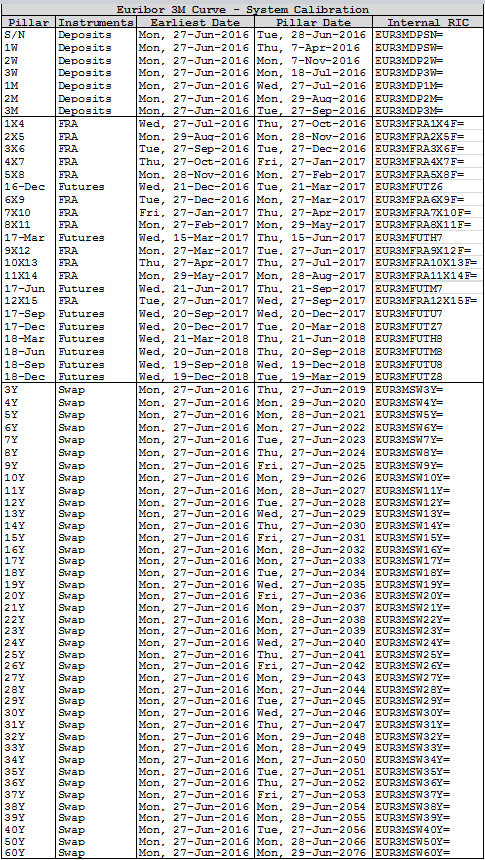
\includegraphics[width=0.58\textwidth]{images/3MMx.png}
\caption{Bootstrapping instruments selected for System calibration of Euribor 3M Curve and corresponding Internal RICs (Evaluation Date 30 October 2015)}
\label{fig:3MMx}
\end{figure}

\section{6M Curve}

\subsection{Excel Calibration}

6M Euribor curve is bootstrapped using the following instruments:
\begin{itemize}
\item Synthetic Deposits from 1M to 6M; 
\item FRAs up to 2Y;
\item 6M Swaps up to 60Y;
\item two Forward Swaps with tenor 30Y to cover 45Y and 55Y maturities.
\end{itemize}
The curve structure with corresponding Market RICs is shown in Figure \ref{fig:6MExcel}.

\begin{figure}
\centering
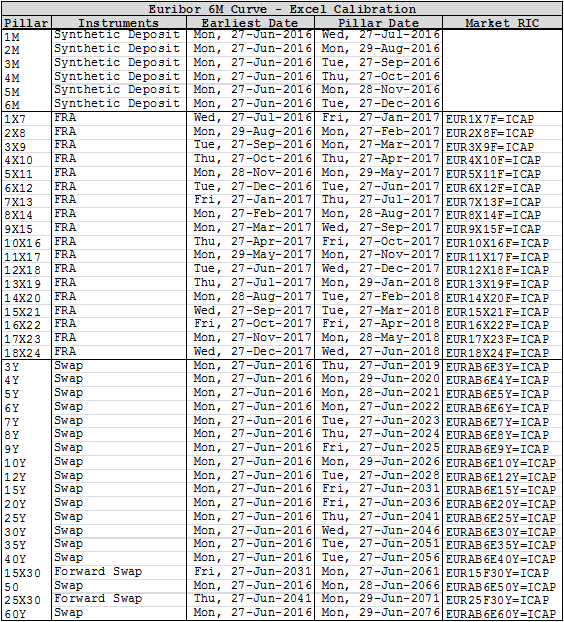
\includegraphics[width=0.58\textwidth]{images/6MExcel.png}
\caption{Bootstrapping instruments selected for Excel calibration of Euribor 6M Curve and corresponding Market RICs (Evaluation Date 30 October 2015)}
\label{fig:6MExcel}
\end{figure}

\subsection{System Calibration}

The curve structure with corresponding Internal RICs is shown in Figure \ref{fig:6MMx}. The contribution instruments are listed below:
\begin{itemize}
\item Deposits from SN to 6M maturity; 
\item FRAs up to 30M;
\item 6M Swaps up to 60Y.
\end{itemize}
Notice the presence of one additional synthetic interpolated FRA (in addition to interpolated deposits and swaps): as said before, we have to lock as many pillars as possible to be able to use Kruger interpolation, which guarantees stable deltas, and obtain good forward rates.  

\begin{figure}
\centering
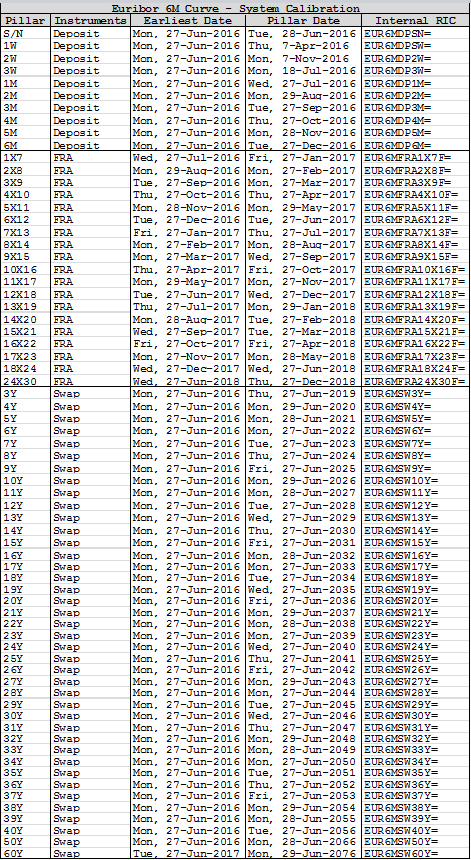
\includegraphics[width=0.58\textwidth]{images/6MMx.png}
\caption{Bootstrapping instruments selected for System calibration of Euribor 6M Curve and corresponding Internal RICs (Evaluation Date 30 October 2015)}
\label{fig:6MMx}
\end{figure}

\section{12M Curve}

\subsection{Excel Calibration}

12M Euribor curve is bootstrapped using the following instruments:
\begin{itemize}
\item 3M, 6M, 9M, 12 Synthetic Deposits; 
\item FRAs up to 2Y;
\item 6M-12M Basis Swaps up to 60Y.
\end{itemize}
The curve structure with corresponding Market RICs is shown in Figure \ref{fig:12MExcel}.

\begin{figure}
\centering
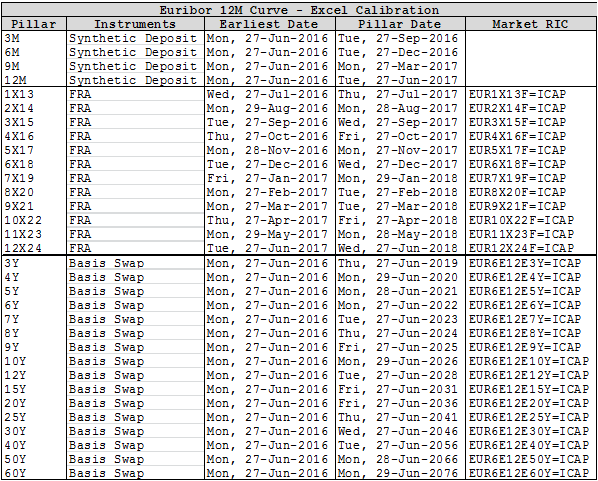
\includegraphics[width=0.58\textwidth]{images/12MExcel.png}
\caption{Bootstrapping instruments selected for Excel calibration of Euribor 12M Curve and corresponding Market RICs (Evaluation Date 30 October 2015)}
\label{fig:12MExcel}
\end{figure}

\subsection{System Calibration}

The curve structure with corresponding Internal RICs is shown in Figure \ref{fig:12MMx}. The contribution instruments are listed below:
\begin{itemize}
\item Deposits from SN to 12M maturity; 
\item FRAs up to 2Y;
\item 12M Synthetic Swaps up to 60Y.
\end{itemize}

\begin{figure}
\centering
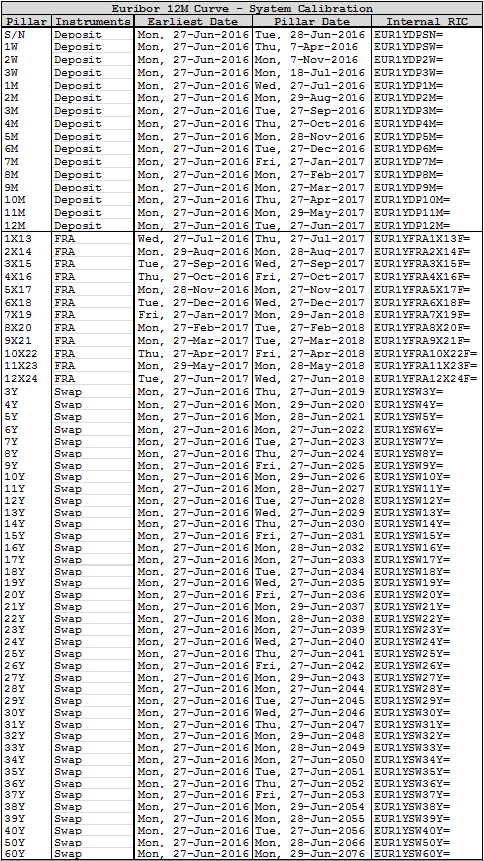
\includegraphics[width=0.58\textwidth]{images/12MMx.png}
\caption{Bootstrapping instruments selected for System calibration of Euribor 12M Curve and corresponding Internal RICs (Evaluation Date 30 October 2015)}
\label{fig:12MMx}
\end{figure}
